% -*- mode:flyspell; mode:latex -*-
% \documentclass[a4paper,twoside,11pt]{book}
\documentclass[12pt]{article}
\usepackage[latin1]{inputenc}
\usepackage[T1]{fontenc}
\usepackage[english]{babel}
\usepackage{graphicx}
\usepackage{float}
\usepackage{amsmath}
\usepackage{hyperref}
\usepackage{hhline}
\usepackage{subfig}
\usepackage{color}
\usepackage[all]{hypcap}
% \usepackage[normalem]{ulem}  % for striking out
% \usepackage{fancyhdr}
% \pagestyle{fancy}
% \fancyhead[C]{}
% \fancyhead[L] {\it{Mu2e-doc-4555-v1.0} }

\usepackage[square,sort,comma,numbers]{natbib}

% \usepackage[backend=biber, style=numeric-comp, sorting=ynt] {biblatex}

% \addbibresource{mu2e_internal_notes.bib}
% \addbibresource{radiative_muon_capture.bib}
% \addbibresource{radiative_pion_capture.bib}

\newcommand {\red}          {\color{red}}
\newcommand {\blue}         {\color{blue}}

\newcommand {\kmax}         {\mbox{$k_{\rm max}$}}
\newcommand {\mubunch}      {$\mu$Bunch}
\newcommand {\MuMinusEPlus} {\mbox{$\mu^- \rightarrow e^+$}}
\newcommand {\ra}           {\mbox{$\rightarrow$}}

\graphicspath{{figures/}}

\begin{document}

\begin{titlepage}
  \begin{flushright}
    \bf {MU2E/PHYSICS/22262} \\
    version 0.0
    \today
  \end{flushright}

  \vspace{1cm}
  
  \begin{center}
    {\Large \bf Understanding the \kmax\ fits of the RMC spectra} 
    
    \vspace{1cm}
    
    E.Diociaiuti (Roma), M.Mackenzie (Northwestern), P.Murat(FNAL)
    
    % \footnote{\texttt{Fermilab; e-mail: murat@fnal.gov}}
    \vspace{0.3cm}
    
    \vspace{0.8cm}                           
  \end{center}

  \begin{abstract}
    
    This note summarizes our effort on understanding the kMax fits of the RMC spectra.

    Mistakes and other internal inconsistencies found in the literature make
    it difficult to rely on the results of other experiments when predicting RMC
    background to the search of mu- -->e+ conversion process.
    
    To reliably predict RMC background to mu- --> e+, Mu2e needs to have its own
    measurement of the endpoint of the RMC photon spectrum on Al.
    
  \end{abstract}

\end{titlepage}
% \frontmatter
% \chapter*{Abstract}
%
% \addcontentsline{toc}{chapter}{Abstract}
%
% \mainmatter
%
{\tableofcontents}

%%%%%%%%%%%%%%%%%%%%%%%%%%%%%%%%%%%%%%%%%%%%%%%%%%%%%%%%%%%%%%%%%%%%%%%%%%%%%%%
%\chapter{Calibration}
%%%%%%%%%%%%%%%%%%%%%%%%%%%%%%%%%%%%%%%%%%%%%%%%%%%%%%%%%%%%%%%%%%%%%%%%%%%%%%%
\section{ RMC as a background to \MuMinusEPlus\ conversion search }
% 
% \begin{figure}[H]
%   \includegraphics[width=1.05\textwidth]{figures/png/beam_flash_electron_momentum} 
% 
%   \caption{
%    momentum spectrum of the beam flash electrons
%   }
% \end{figure}

Radiative muon capture (RMC) is one of the most important backgrounds to the search for
\MuMinusEPlus\ conversion on nuclei. In case of the Mu2e target of choice, aluminum,
RMC is also the most uncertain one: the expected $e^+$ signal energy, E = 92.32 MeV,
is close enough to the endpoint of the RMC spectrum on aluminum,
$90 \pm 2$ MeV \cite{RMC_1999_PhysRevC.59.2853}, so variations of the endpoint
energy within the experimental errors could result in significant changes
in the RMC background expectations.
%
We note that the uncertainty in the RMC background expectations is mostly due to the
published experimental uncertainty of 2 MeV - the Mu2e energy resolution of about 300-400 keV
is small compared to a $\sim$ 3 MeV difference between the expected signal energy
and the maximal energy of a positron coming from a conversion of a RMC photon.
However, given the published 2 MeV uncertainty on the RMC spectrum endpoint the two 
numbers are just about 1.5 standard deviation apart, so understanding of the
experimental uncertainty on \kmax\ becomes quite important.

Fortunately, measurements on the photon spectra on nuclei published 
by the TRIUMF RMC spectrometer group in \cite{RMC_1992_PhysRevC.46.1094},
\cite{RMC_1999_PhysRevC.59.2853} - provide sufficient information for readers
to reproduce the published photon spectrum endpoints, and in this note
we report on our attempt to do so.

The endpoint of the RMC photon spectrum is determined using the closure
approximation model \cite{RMC_1979_CERN_REF-TH-2967}.
In this model, the photon spectrum is fully defined by a single parameter,
the photon spectrum endpoint energy \kmax:
$$
   {dN \over dx} = {e^2 \over \pi} {\kmax^2 \over {m_\mu^2}}  (1-x) (1-2x+2x^2) x (1-x)^2
$$
, where $x = k/\kmax$.

We use parameterizations of the TRIUMF RMC spectrometer response
to convolute them with the closure approximation spectra, fit the experimental data,
determine the best \kmax\ values and the corresponding fit uncertainties
for different nuclei, and compare the fit results to the published values.

%%%%%%%%%%%%%%%%%%%%%%%%%%%%%%%%%%%%%%%%%%%%%%%%%%%%%%%%%%%%%%%%%%%%%%%%%%%%%%%
\section { Parameterization of the Detector Response}


Published are the measured data. To compare them to the model predictions,
one needs to know how the theoretical spectrum is modified by the detector
response, i.e. know the detector response.

Fortunately, references  \cite{RMC_1992_PhysRevC.46.1094}, \cite{RMC_1999_PhysRevC.59.2853}
have the detector response published.

Also published is the RPC spectrum on $H_2$ used for calibration.

We check how well different parameterizations of the detector response describe the
calibration peak.
\begin{figure}[htbp]
 \begin{center}
 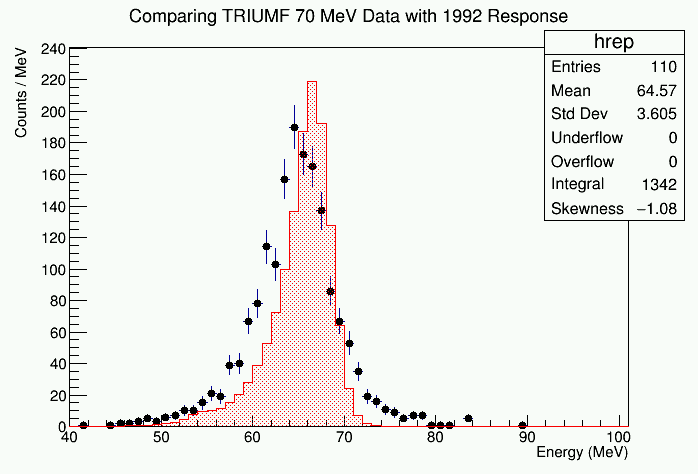
\includegraphics[width=0.49\columnwidth]{png/70MeV_vs_1992_Response} 
 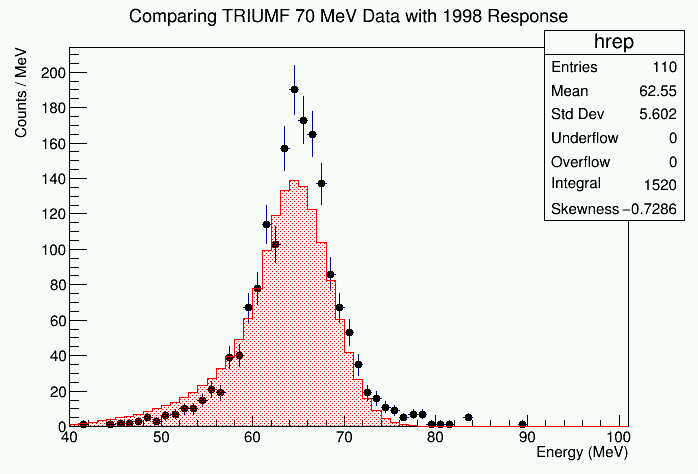
\includegraphics[width=0.49\columnwidth]{png/70MeV_vs_1998_Response} 
 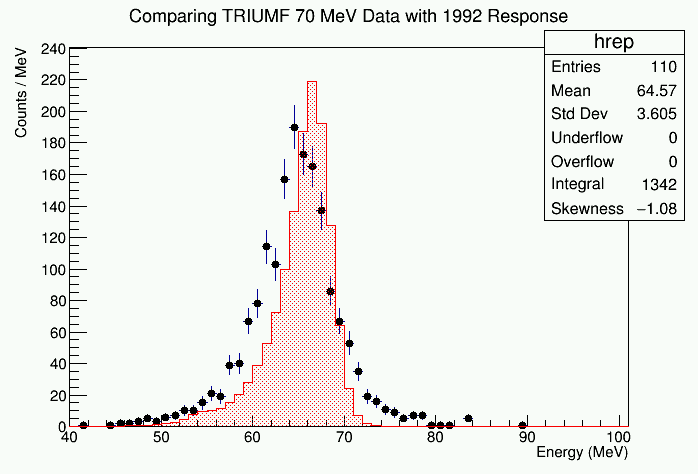
\includegraphics[width=0.49\columnwidth]{png/70MeV_vs_1992_Response} 
 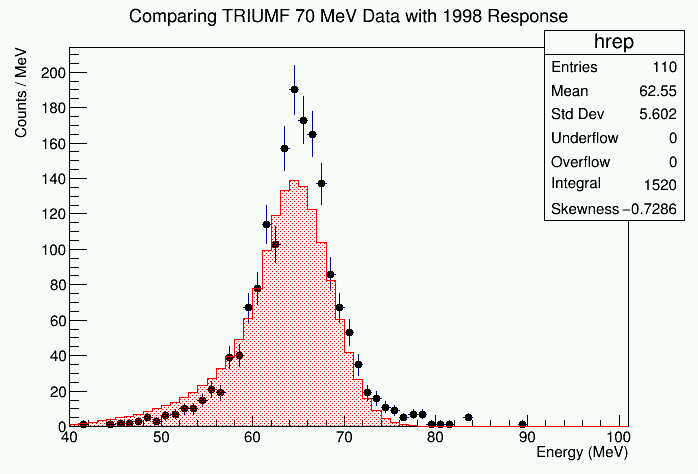
\includegraphics[width=0.49\columnwidth]{png/70MeV_vs_1998_Response} 
 \end{center}
 \caption{\red{ \bf Caption}}
 \label{p004}
 \end{figure}

%%%%%%%%%%%%%%%%%%%%%%%%%%%%%%%%%%%%%%%%%%%%%%%%%%%%%%%%%%%%%%%%%%%%%%%%%%%%%%%
\section { Input Data for fits}

Input data used are the digitized figures from references
\cite{RMC_1992_PhysRevC.46.1094,RMC_1999_PhysRevC.59.2853}.

\begin{figure}[htbp]
 \begin{center}
 
\includegraphics[width=0.7\columnwidth]{png/missing_plot} 
 \end{center}
 \caption{\red{ \bf Caption}}
 \label{p004}
 \end{figure}
Checks of the digitization accuracy

Errors - statistical. Systematic uncertainty on the energy scale in the
published data - less than 0.5 MeV.

%%% Local Variables:
%%% mode: latex
%%% TeX-master: "."
%%% End:

%%%%%%%%%%%%%%%%%%%%%%%%%%%%%%%%%%%%%%%%%%%%%%%%%%%%%%%%%%%%%%%%%%%%%%%%%%%%%%% 
% %%% Local Variables:
%%% mode: latex
%%% TeX-master: "."
%%% End:
\section { Fits }


%%%%%%%%%%%%%%%%%%%%%%%%%%%%%%%%%%%%%%%%%%%%%%%%%%%%%%%%%%%%%%%%%%%%%%%%%%%%%%
\subsection { Fits of the 1992 data }

%%%%%%%%%%%%%%%%%%%%%%%%%%%%%%%%%%%%%%%%%%%%%%%%%%%%%%%%%%%%%%%%%%%%%%%%%%%%%%
\subsection { Fits of the 1995 data }

%%%%%%%%%%%%%%%%%%%%%%%%%%%%%%%%%%%%%%%%%%%%%%%%%%%%%%%%%%%%%%%%%%%%%%%%%%%%%%
\subsection { Fits of the 1998 data }

%%%%%%%%%%%%%%%%%%%%%%%%%%%%%%%%%%%%%%%%%%%%%%%%%%%%%%%%%%%%%%%%%%%%%%%%%%%%%%
\subsection { Fits of the 1999 data }


%%%%%%%%%%%%%%%%%%%%%%%%%%%%%%%%%%%%%%%%%%%%%%%%%%%%%%%%%%%%%%%%%%%%%%%%%%%%%%%
\section { Discussion }

\begin{enumerate}
\item
  Our fits result in significantly smaller errors on kMax. It seems very likely
  that the TRIUMF RMC spectrometer collaboration used wrong definition of the
  fit errors. Plot on page 45 from reference \cite{BERGBISH_MS_THESIS} indicates
  that the fit error has been defined as the change in the parameter value,
  corresponding the the change in the fit $\chi^2/DOF$ by 1, rather than to the change
  by one in the total fit $\chi^2$. The number of bins in the fit histograms
  is about 35-40 is consistent with our fit errors being 5-6 times smaller than
  the published ones.
\item
  '1999 parameterization of the detector response gives significantly better
  fits of all spectra published by the TRIUMF RMC spectrometer 
  ('1992, '1995, '1998, and '1999)
\item
  chi2's of the fits with '1992 response are large enough to suggest wrong
  parameterization. Our chi2's per degree of freedom are consistent with
  the published ones
\item
  However, the '1992 response is consistent with the RPC peak published
  in 1992, while '1998 response - is not. This confirms internal consistency
  of the '1992 publication 
\item
  different kMax fits for the same target vary on a scale large compared
  to the fit errors
\item
  how our fit results are different from the published? 
\end{enumerate}

% \newpage
%%%%%%%%%%%%%%%%%%%%%%%%%%%%%%%%%%%%%%%%%%%%%%%%%%%%%%%%%%%%%%%%%%%%%%%%%%%%%%%
\section{ Summary }


The only thing we can claim for certain is that the fit uncertainties on kMax are
of the order of 0.5 MeV, not 2 MeV. Published uncertainties of about 2-3 MeV
have been derived using wrong procedure (fit of the distribution of chi2/dof
instead of the total chi2)


For Al, the fit results are consistent with the published - about 90 MeV.


Plan : use aluminum data

a)Assume $90 \pm 0.5$ MeV, determine the RMC background

b) assume kMax + 3 sigma, determine the RMC background

%%%%%%%%%%%%%%%%%%%%%%%%%%%%%%%%%%%%%%%%%%%%%%%%%%%%%%%%%%%%%%%%%%%%%%%%%%%%%%% 
\section{ Acknowledgements }

We want to thank ...

%%%%%%%%%%%%%%%%%%%%%%%%%%%%%%%%%%%%%%%%%%%%%%%%%%%%%%%%%%%%%%%%%%%%%%%%%%%%%%
     %% 
     %% % \addcontentsline{toc}{chapter}{Bibliography}
     %
\bibliographystyle{plain}
\bibliography{radiative_muon_capture}

% \printbibliography
\end{document}


% ------------------------------------------------------------------------------
% templates
% ------------------------------------------------------------------------------
% Table ~\ref{table:summary} gives summary the numbers used in this study.
% 
% \hspace{-0.1in}
% \begin{table}[htbp]
%   \label{table:summary}
%   \begin{center} 
%     {\renewcommand{\arraystretch}{1.0}   % change 1.0 to 1.1 to increase the spacing between the table lines
%       \begin{tabular}{|c|c|c|c|}
%         \hline
%                             & default TS geometry & misaligned TS geometry   &  Ratio(default/misaligned)    \\ 
%         \hline
%         $N_{POT}$            &  $4.96 \cdot 10^6$  &    $5.00 \cdot 10^6$      &   0.992   \\ 
%         $N_{\mu}^{TS3u}$      &  65648              &     61354                 &   1.070   \\ 
%         $N_{\mu}^{TS5}$       &  28517              &     27351                 &   1.043   \\ 
%         $N_{\mu}^{ST}$        &  8868               &      8396                 &   1.056   \\ 
%         $N_{\mu}^{ST}/N_{POT}$ &  $1.79 \pm 0.02$    &    $1.68 \pm 0.02$        &   $1.065 \pm 0.03$        \\ 
%         \hline
%       \end{tabular}
%     }
%   \end{center}
%   \caption{
%     Muons rates at different points of the Mu2e beamline and stopping muon rates for nominal and 
%     misaligned TS geometries
%   }
%   % \vspace{0.5in}
% \end{table}
